\subsubsection{The Problem of Overfitting}
\begin{itemize}[--]
	\item \textbf{Underfitting}: when a model cannot capture the underlying trend of the data ("high bias")
	\item \textbf{Overfitting}: when a model captures the noise of the data ("high variance")
	\item \textbf{Generalize}: fails to fit to new examples
	\item Overfitting's poor generalization results in low costs not always being correct
	\begin{center}
		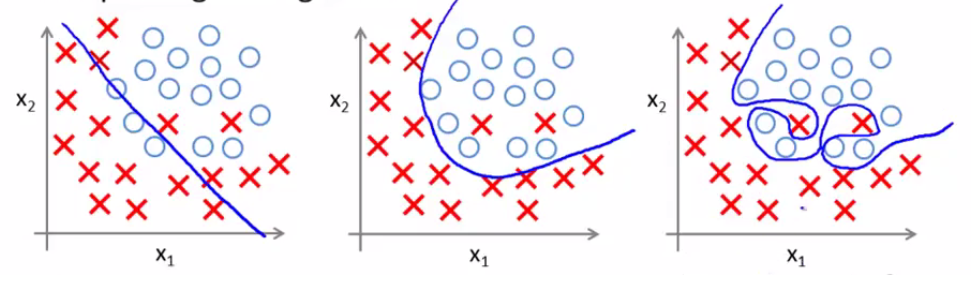
\includegraphics[scale=0.5]{sections/cs229/w4/over-under.png}
	\end{center}

	\item If we have too many features for very little data, overfitting can easily become a big problem.
	\item Options:
	\begin{itemize}
		\item Reduce number of features
		\begin{itemize}
			\item Manually select which features to keep
			\item Model selection algorithm (later in course)
		\end{itemize}
		\item Regularization
		\begin{itemize}
			\item Keep all the features, but reduce magnitude/values of parameters $\theta_j$
			\item Works well when we have a lot of features, each of which contributes a bit to predicting $y$
		\end{itemize}
	\end{itemize}

\end{itemize}

\subsubsection{Cost Function}
\begin{itemize}[--]
	\item Having smaller values for parameters $\theta_0, \theta_1, \ldots, \theta_n$
	\begin{itemize}[--]
		\item ``Simpler'' hypothesis
		\item Less prone to overfitting
	\end{itemize}

	\item To exemplify lets consider the housing scenario:
	\begin{itemize}[--]
		\item Features: $x_1,\ldots, x_100$
		\item Paremeters: $\theta_0, \ldots, \theta_100$
		\item We don't know which ones are complex to shrink, so we modify the cost function to shrink every parameter
		$$J(\theta )=\frac{1}{2m}(\sum_{i=1}^{m}(h(x^{(i)}-y^{(i)})^2 + \lambda\sum_{i=1}^{n}\theta_j^2)$$
		\item We don't penalize $\theta_0$ by convention, because it's a constant and makes very little difference
	\end{itemize}

	\item $\lambda$ is called the regularization parameter. It controls the trade off of fitting the training set well and keeping the parameters small and simple to prevent overfitting
	\item If $\lambda$ is set to be very large we will penalize all the paramters extremely highly resulting which will result in all by the constant being close to zero (fits to a horizontal line). ``Underfit''
\end{itemize}

\subsubsection{Regularized Linear Regression}
\begin{itemize}[--]
	\item Using the new regularized linear regression cost function from the previous section we can now update our gradient descent algorithm to encorporate this modification:
		$$\theta_0 := \theta_0 - \alpha\frac{1}{m}\sum_{i=1}^{m} (h(x^{(i)})-y^{(i)})x_0^{(i)}$$
		$$\theta_j := \theta_j - \alpha ( \frac{1}{m}\sum_{i=1}^{m}(h(x^{(i)})-y{(i)})x)j^{(i)} +\frac{\lambda}{m}\theta_j )$$

	\item The $\theta_j$ $(j=1,\ldots, n)$ term can also be written:
		$$\theta_j := \theta_j (1-\alpha\frac{\lambda}{m}) - \alpha\frac{1}{m}\sum_{i=1}^{m}(h(x^{(i)}) - y^{(i)})x_j^{(i)}$$

	\item The term $(1-\alpha\frac{\lambda}{m})$ is typically $<1$, so this results in shrinking $\theta_j$ by multiplying by a value $<1$, and then performing the same gradient descent function
	\item We also had the normal equation to solve the same problem, and it can also be updated for regularization:
		$$\theta = (X^{T}X+\lambda \left[ \begin{smallmatrix}
			0 & & &\\
			& 1 & &  \\
			& & \ldots & \\
			& & & 1 
		\end{smallmatrix}\right] )X^{T}y$$

	\item Suppose $m\leq n$ then $(X^{T}X)$ will be non-invertible/singular
	\item Regularization will take care of this flaw so long as $\lambda > 0$
\end{itemize}

\subsubsection{Regularized Logistic Regression}
\begin{itemize}[--]
	\item We can also regularize logistic regression in a similar manner
		$$\theta_0 := \theta_0 - \alpha\frac{1}{m}\sum_{i=1}^{m} (h(x^{(i)})-y^{(i)})x_0^{(i)}$$
		$$\theta_j := \theta_j - \alpha ( \frac{1}{m}\sum_{i=1}^{m}(h(x^{(i)})-y{(i)})x)j^{(i)} +\frac{\lambda}{m}\theta_j )$$
		$$h(x)=\frac{1}{1+e^{-\theta^{T}x}}$$
\end{itemize}